%
% Documento: Disposições
%

\chapter{DESENVOLVIMENTO PROPOSTO}\label{chap:proj}
    O \textit{framework} proposto é baseado no conceito de \textit{PageObject}, onde todas as páginas web são tratadas como objetos.
    Ainda, cada componente que seja necessário para automação, um \textit{input}, \textit{span}, etc, é um atributo desse objeto.

    Para melhor exemplificar o uso do conceito de \textit{PageObject} será utilizado como exemplo um simples \textit{login} para 2
    usuários, onde será utilizada uma página que possui dois campos de texto, campo de usuário e outro de senha,
    e um botão para submeter o \textit{login}.

    Primeiramente se utilizou de um exemplo básico de como o \textit{Selenium} propõe o desenvolvimento desse \textit{script} de
    \textit{login}. No começo é iniciado o \textit{driver} do navegador, navegar para a \textit{URL}, depois
    são seguidos 3 passos para cada um dos campos de texto, procurar por ele, limpar o seu conteúdo
    (porque não se sabe se ele possui algum texto pré cadastrado) e enviar os caracteres necessário para
    cada campo e por final, procurar e clicar no botão para submeter a ação do formulário. Não é um método muito viável,
    pois caso tenhamos 2 \textit{logins} esse \textit{script} deverá ser duplicado para atender ambas necessidades.

    Num segundo exemplo poderíamos separar o \textit{script} de \textit{login} e criar um módulo separado para ele. Desse jeito
    os \textit{scripts} podem fazer uso do mesmo código e caso uma terceira pessoa precise dele não seria um problema.
    Porém temos todo o mapeamento dessa página está preso num módulo e caso seja necessário a criação de outro
    módulo que use essa mesma página ainda assim teremos que duplicar mais código.

    Chegando num terceiro exemplo onde agora fazemos uso do \textit{framework} \textit{Pybot}, onde utilizando-se do
    módulo \textit{Component} (\autoref{sec:comp}) podemos separar todos os componentes da tela em atributos da nossa página
    e criar um método onde precisando de dois parâmetros ele faz o processo de \textit{login}, e ainda assim, caso
    necessário pode-se utilizar os campos mapeados para fazer algum outro método sem impactar o \textit{login}.
    E caso alguma referência dos campos mapeados mude, será necessário alterar apenas um local e nenhum \textit{script}
    será impactado.


    Para exemplificar esses cenários mostrados foram feitos alguns diagramas que estão presentes no \autoref{app:imgs}, onde:
    Na \autoref{fig:selenium_default} exemplifica o primeiro cenário mostrado, onde temos dois usuários com \textit{scripts} de \textit{login}
    idênticos, porém cada com a sua implementação;
    Na \autoref{fig:selenium_module} exemplifica o segundo cenário mostrado, onde agora temos um \textit{script} de \textit{Login}
    separado dos \textit{scripts} de cada usuário, porém ainda temos toda o mapeamento da página preso num único script;
    Na \autoref{fig:pybot_module} exemplifica o terceiro cenário mostrado, onde com o uso do \textit{Pybot} a página de \textit{login}
    é tratada como um objeto e dentro dela temos o método \textit{login} para ser usado nos \textit{scripts} de cada usuário.


    Tendo isso em mente é possível entender uma das vantagens do uso do \textit{PageObject} para criação dos \textit{scripts} que
    o \textit{Pybot} faz uso, e com isso analisar como ficaria a implementação desse \textit{scripts} dos exemplos, fazendo uso apenas
    do \textit{Selenium}, primeiro cenário mostrado, e outro usando o \textit{Pybot}, terceiro cenário mostrado.

    A \autoref{fig:exemplo_selenium} mostra o uso do \textit{Selenium} onde temos toda a execução e os comandos do \textit{script} em
    apenas um arquivo. Seus comandos são simples e bem verbosos, tornando assim o script de fácil entendimento das ações que serão executadas.
    No início do codigo é feita a importação do \textit{framework}, seguido da iniciação do navegador \textit{Firefox} (caso o \textit{driver} esteja nas
    variáveis de ambiente da máquina da execução), seguido da pesquisa, limpeza e preenchimento dos valores para os campos de texto, seguido da pesquisa
    e \textit{click} no botão e por fim o encerramento do \textit{script}. Ele resolve o cenário dos usuários descrito anteriormente, mas não dá assim a
    flexibilidade da criação de outros scripts com o aproveitamento de código.


    \begin{figure}[H]
        \vspace*{0,5cm}
        \centering
        \caption{Exemplo de uso com Selenium}
        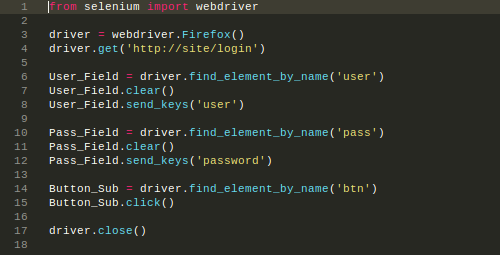
\includegraphics[width=0.9\textwidth]{./04-figuras/exemplo_selenium}
        \label{fig:exemplo_selenium}
        \vspace*{0,5cm}
    \end{figure}

    Agora na \autoref{fig:exemplo_pybot} temos um código fazendo uso do \textit{Pybot}. Com ele foi feita a separação do codigo da página de
    \textit{login} em outro arquivo, e com o uso da classe \textit{PageObject} para a criação da nossa página e dentro dela utilizado a classe de
    \textit{PageElement} para o mapeamento dos elementos da página, dessa maneira o codigo fica mais organizado e agora temos um contexto sobre
    onde cada elemento definido pertence. Junto da classe de \textit{Login} foi feita a definição de um método de login que faz o uso dos \textit{PageElements}
    para a atribuição dos valores nos campos de texto seguido do \textit{click} do botão. Utilizando o \textit{Pybot} o código responsável pelo login
    fica totalmente independente dos \textit{scripts}, e os mesmo se tornam muito mais simples e diretos para mostrar o seu propósito. Com isso o script ficou
    muito menor e simples sendo necessário apenas fazer a importação do próprio \textit{Pybot} para dar início ao \textit{script} e da página de login para utilizar-se do método.

    \begin{figure}[H]
        \vspace*{0,3cm}
        \centering
        \caption{Exemplo de uso com Pybot}
        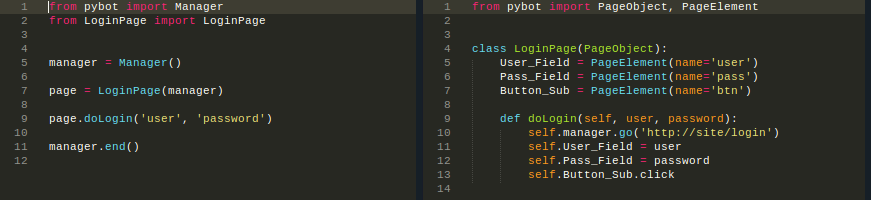
\includegraphics[width=1\textwidth]{./04-figuras/exemplo_pybot}
        \label{fig:exemplo_pybot}
    \end{figure}




